\chapter{Software System}
\label{software_system}
In this Chapter, we discuss the development of the software system used to conduct the experiments described later in this thesis. First, we describe the basic requirements for such a system and then go into the ``story'' behind the development, show where we were stuck and how we solved these problems. Then we are going to describe the environment in which this software system can be used and what kind of external software and hardware was used to run the experiments on.

\section{Requirements}
We started the development of the system by defining which requirements it has to fulfill in order to be suitable for conducting the experiments of this thesis. The following properties were identified which the developed system should fulfill:

\begin{itemize}
	\item \textbf{Parameterizable}: All experiments should be allowed to run in parameterized manner, which means that all important hyperparameters, training samples and places to store the different results should be parameterizable through a JSON\footnote{http://www.json.org/} configuration file.
	\item \textbf{Repeatable}: It should be possible to run experiments multiple times without having to put additional efforts into it.
	\item \textbf{Analyzable}: This means that all results from all experiments should be stored in a distinct place for analysis later. This includes the trained models, all metrics collected while training and also the configuration used.
	\item \textbf{Recoverable}: Due to the fact, that we knew that the environment in which the experiments were going to be conducted (see Chapter \ref{software_system:hardware} on the hardware) is unstable, we decided that we must design the system in such a way that we should easily be able to recover from the premature termination of an experiment. This means, that it should be possible to load the most recent model from the previous training and go on from the point where the training was interrupted. This includes loading and saving of the model weights, skipping all of the samples dataset the model was already trained on as well as loading all the metric already collected in the first run.
	\item \textbf{Evaluable}: The trained models should be easily evaluable, which means that we should have a way of doing inference without the hassle to load the stored configurations and models by hand. The most comfortable way of doing this is through a small frontend which provides the possiblity to communicate with a trained model.
\end{itemize}

The properties listed above should be fulfilled by the newly developed system in order to enable us to safely conduct experiments without the fear of loose any of the results.

\section{Development of the System}
\label{sofware_system:development_history}
In this Chapter, we want to give an insight on the development on the software system and shed light on some decision we have made in the process.

\paragraph{Switch from Keras to TensorFlow} The first and probably also the largest decision we had to make was, if we would remain with \texttt{keras}\footnote{https://keras.io/} as our deep learning framework or if we switch to \texttt{TensorFlow}\footnote{https://www.tensorflow.org/}. We already had developed a software system for conducting experiments with \texttt{keras} in the context of our ``Projektarbeit'' in the autumn semester of 2016, even thought this system was used to perform sentiment-analysis with convolutional neural networks \cite{Vongruenigen:2017}. But, from that experience, we also knew that \texttt{keras} is a pretty high-level framework with a lot of abstractions to hide the tedious details from the user. This is beneficial for getting up-and-running quickly, but we wanted to get further insight on how these models actually work and how they are implemented, especially with a computational graph, as this seems to be a pretty common technique to build such systems these days \cite{TensorFlow:2015}\cite{Theano:2016}\cite{Torch:2011}.

Due to the urge to get more detailed knowledge, we decided to opt for \texttt{TensorFlow} as our framework of choice instead of \texttt{keras}, even though the implementation would probably have been easier using the latter.
\paragraph{Beginning Was Hard} We had to spend the first few weeks to get some basic knowledge about sequence-to-sequence learning and \texttt{TensorFlow} and how its internal graph works. The learning curve was really steep at the beginning, especially when talking about managing the computational graph. In \texttt{keras}, everything related to the graph of \texttt{theano} is hidden behind abstractions and the user of the framework rarely has to implement a functionality by itself. This is the complete opposite in \texttt{TensorFlow}: Most of the time developing the model is spent on the implementation of the graph and even when using specialized seq2seq APIs provided, it took a long time to get used to regardless. After our first few experiences with \texttt{TensorFlow} in general, we started to concentrate on the model we wanted to implement.

So we started by using the API in the namespace \texttt{tf.contrib.seq2seq} as this seemed to be the one which is under development currently. The implementation itself took around one to two weeks and we started a training with this new model directly after we finished the implementation. After the training had finished, we started to do inference to shockingly notice that the model does not seem to work. The outputs of the model itself were nonsense as they were texts, where it seemed to choose random words and repeat them for a random number of times. We started by analyzing our implementation in detail, but could not find the obvious problem. Driven by the problem, we started to do a research on which of the seq2seq APIs was usable and quickly found out, that the API we thought we were going to use, was unmaintained and we could not seek out to anybody for help regarding our problem.

\paragraph{Ongoing Problems} After realizing that the first API we had chosen was not sufficient, we started to search the internet for a solution on which seq2seq API we could use or if we had to implement the whole system by ourself. That was the moment when we noticed, that Google had released a framework\footnote{https://github.com/google/seq2seq} specifically for seq2seq models with \texttt{TensorFlow}. Of course we were excited to try it out and so we started with conducting experiments using the framework some days later. At first, everything looked fine and the training seemed to be working by the look of it. We trained a model on the OpenSubtitles corpus and assumed that we could do the first tests by doing inference a few days later. The first problem we faced was, that it was not possible to do any validation while training the model. This had to do with a bug\footnote{https://github.com/google/seq2seq/issues/103} that also troubled us later when doing inference. We nevertheless started training in the hope that this would only be a temporary bug and would not affect us for a prolonged period of time. We were wrong with this assumption, because it took about a month to fix the issue completely, as it was not only caused by a bug in the framework but by a bug in \texttt{TensorFlow} itself. Due to this bug, we were also not able to do inference on a trained model, which worsened our situtation even more.

Due to the problems pointed out above, we decided that we would better switch back to our own implementation for the model instead on relying on a framework with serious bugs and flaws which did not seem to be solved in a predictable time frame.

\paragraph{Finally a Working Model} We knew that our own implementation also had bugs, but we were eager to find and fix them. We started by reiterating the implementation of the model on the \texttt{TensorFlow} and noticed, that we had made a colossal mistake which was present in all our implementations before: We \emph{always} initialized the graph with random values when starting an experiment. This is the usual procedure when creating a \emph{new} \texttt{TensorFlow} model, but it is a severe mistake when we are doing that after an already trained model has been loaded. So we went on to fix this problem. Our second problem was, that we had no clue on how experimental and stable the seq2seq APIs from \texttt{TensorFlow} are. After some more research, we found an example of a working model in a tutorial of the \texttt{TensorFlow} team on how to implement a simple neural machine translation system using their framework\footnote{https://www.tensorflow.org/tutorials/seq2seq}. This implementation however relied on a deprecated API in the namespace \texttt{tf.contrib.legacy\_seq2seq}. We implemented the model and decided, that we somehow had to validate that the model was working as expected. This was the time, when we started to wrap our heads around model validation tests. We came up with two, an overfitting and a copy task, with which we decided to validate our models from now on. It took us two to three days to develop these tests and another day or two for validating the latest model. After these tests were successful, we decided that we would use the latest model using the deprecated API from now on, because in the meantime we have found several other projects using the same API successfully.

However, we still had problems due to the sheer size of the model we wanted to run. To reproduce the results from \cite{Vinyals:2015}, we tried to make our model as big as possible to come as close to the used 4096 hidden units and 100k vocabulary. This caused another kind of problem, due to the softmax at the end of the decoder. Since the model was so large, the softmax weights matrix alone would have been around 30 to 40 gigabytes in size, which did not fit on any GPU we knew about at the time. To fix this problem at training time, we started to implement sampled softmax as also mentioned in the tutorial for the model we have chosen to use. This caused another chain of problems due to the fact, that the tutorial was written for older version of the \texttt{TensorFlow} framework prior to the one we were using at the time, which meant, that the implementation in our case would be different. After some research and several days of trial-and-error, we managed to fix the problem and start a training using a model with 2048 hidden units and a vocabulary consisting of 50k words. The training run fine and after a few days we had a trained model on our hands and we wanted to start to do inference.

When we started to do inference with our first, successfully trained model, we quickly noticed that our fix for the problem with the size of the softmax weights matrix was only applicable for training time, because at inference time, the model needs the whole softmax weights matrix to do predictions. This led to ourself revisiting the problem and trying to find a solution for it. We found one in the form of an output projection (similar to the one used in \cite{Vinyals:2015}), which allowed us to project the last hidden state of the decoder down to 1024 units before feeding it to the softmax layer. This meant, that the softmax weights matrix would be halved in size, which allowed us to run the model on a single GPU without having the out-of-memory problem we have faced before. The implementation of this feature was rather tedious, as we had to adapt the existing seq2seq API inside the \texttt{TensorFlow} framework. But we managed to do it and it allowed us to solve the problem with the too large softmax weights matrix when doing inference on a GPU.

The last part which we implemented for our model was the beam-search. As we did not have much prior experience with a computational graph, this task was much harder to pull off than the others before. We were lucky and found several implementations for it scattered throughout the internet\footnote{https://github.com/google/seq2seq/blob/master/seq2seq/inference/beam\_search.py}\footnote{https://github.com/wchan/tensorflow/blob/master/speech4/models/las\_decoder.py}\footnote{https://gist.github.com/nikitakit/6ab61a73b86c50ad88d409bac3c3d09f}\footnote{https://github.com/stanfordmlgroup/nlc/blob/master/decode.py}. They helped us a lot in understanding on how beam-search works in the context of a decoder in a seq2seq model. We managed to implement it with the help of an implementation for an older \texttt{TensorFlow} version\footnote{https://github.com/pbhatia243/Neural\_Conversation\_Models/blob/master/my\_seq2seq.py}. It was quite a struggle to adapt it to the newer \texttt{TensorFlow} version we were using, but we managed to do it.

\paragraph{Summary} In summary, our journey to developing a working seq2seq model for our thesis has brought us fun, pain and knowledge, all at the same time. It was a big struggle in the beginning, where we did not find a way to develop a working model and were disappointed by the seq2seq framework we thought would be our savior. The most interesting part of this came after we were able to put our hands on a working model: The implementation of features surrounding the problem of a ''too big'' model has brought us a lot of joy gave us a lot of insights on how to develop such systems with low-level computational graph operations. The implementation of the beam-search and the down-projection of the hidden state was the by fast the most interesting part, as we had the possibility to work on interal code from the \texttt{TensorFlow} framework which further deepened our knowledge.

\section{Model Validation Checks}
\label{software_sytem:model_validation_checks}
As described in the Section before, we were struggling with the development of the software system, especially with the construction of the \texttt{TensorFlow} graph itself. We have had a lot of setbacks and hence, were not sure how to validate that our latest model is working without spending several days to weeks on training before noticing that the graph is still broken. For this reason, we have developed two so-called model validation checks, which should ensure that the model is not broken before starting the large, long-running experiments.

The first validation we introduced was a simple copy-page task: The model was trained to copy sequences of integers of different lengths. For this purpose, we have generated a dataset of $10,000$ sequences of random length and random content. We have used the integers from $0$ to $19$ as the vocabulary and the generated sequences were between $1$ and $40$ symbols long. We then used the implemented model and trained it to output the exact input sequence, for which we used the aforementioned random integer sequences. 

The second validation was a simple overfitting test: The model was fed with tweets as input sequences and the respective response as output sequences. For this purpose we have used a dataset of english tweets borrowed from the user ''Marsan-Ma'' on GitHub\footnote{https://github.com/Marsan-Ma/chat\_corpus/}. We conditioned the model to output the expected output sequence each time we have used a specific input sequence.

Through using these two validation checks, we were able to gain confidence that the implemented model works as expected without using as much time as a full training on any of the conversational datasets would have required.

\section{Web-UI}
We have also developed an elementary GUI for doing inference through a web frontend. This allowed us to interact with the models after they have been trained in a quick and easy way. We have used the python web framework \texttt{flask}\footnote{http://flask.pocoo.org/} for implementing the backend system and a combination of \texttt{jQuery}\footnote{https://jquery.com/} JavaScript library and the \texttt{boostrap}\footnote{http://getbootstrap.com/} frontend framework.

\begin{figure}[H]
	\centering
	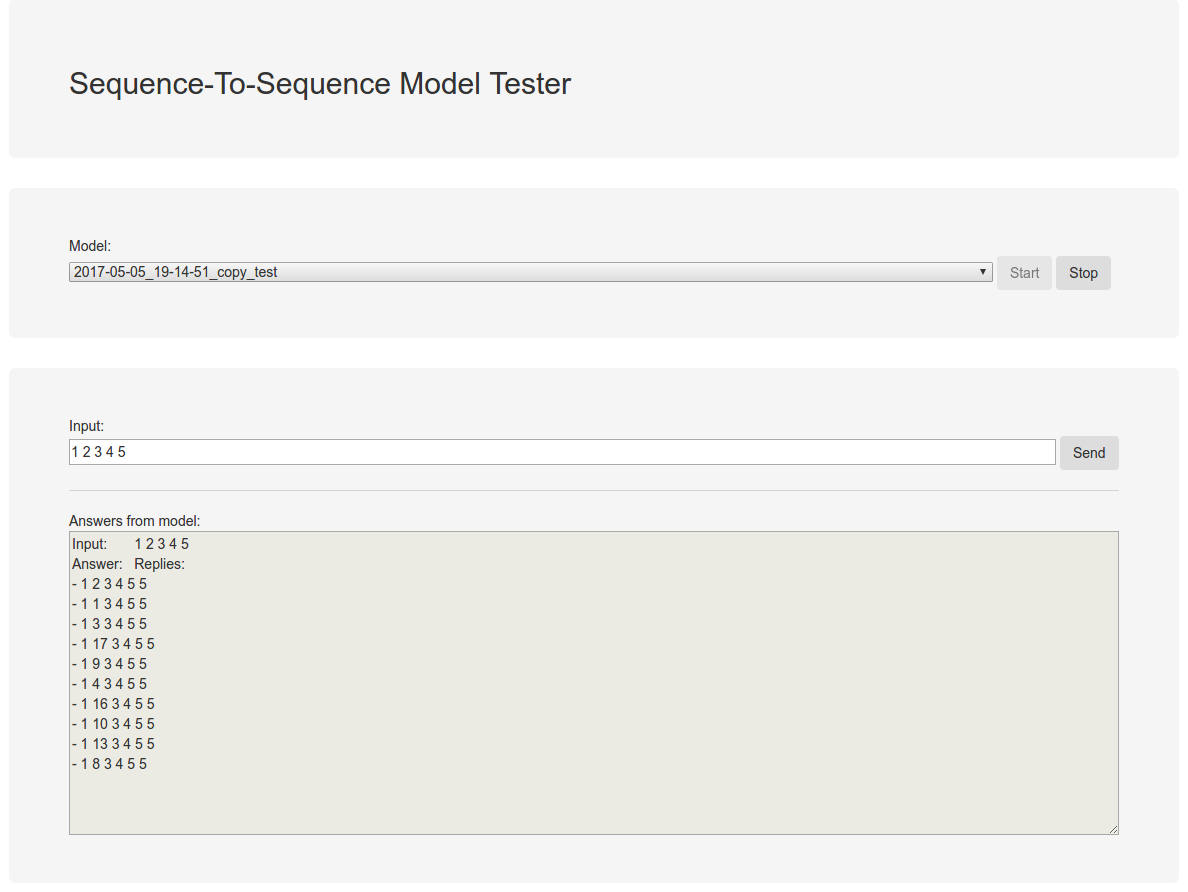
\includegraphics[width=10cm]{img/web_frontend_inference}
	\caption{Frontend showing the output when sending the sequence ``1 2 3 4 5'' to a model trained on the copy task (see Chapter \ref{software_sytem:model_validation_checks}).}
\end{figure}

\section{Scripts}
We have written several scripts in order to prepare, conduct and analyze experiments. These scripts cover, amongst other things, the following functionality:

\begin{itemize}[noitemsep]
	\item Scripts for generating plots of the learning curves and metrics.
	\item Scripts for analyzing the internal structure of the model.
	\item Scripts for preprocessing the training dataset and generating required auxiliary files (e.g. vocabularies).
	\item Scripts for visualizing highly-dimensional data, such as word-embeddings and thought vectors.
	\item Scripts for visualizing the attention mechanism.
	\item Scripts for generating and managing experiments.
\end{itemize}

More informations about the important scripts and details on how to use them can be found in the appendix \ref{appendix:software_usage} on how to use the software system.

\section{Hardware}
\label{software_system:hardware}
All experiments have been conducted on the GPU-cluster the InIT (Institut für angewandte Informationstechnologie) has provided us for running the experiments related to our thesis. On this server, 8 Nvidia Titan X (Pascal) GPUs are installed and a total of 24 CPUs with 501GB of RAM stood at our disposal. The experiments themselves were run in a virtualized manner by using \texttt{docker}\footnote{https://www.docker.com/} with the specialized \texttt{nvidia-docker}\footnote{https://github.com/NVIDIA/nvidia-docker} appliance to ease the integration of the physical hardware into the virtual machine. Most of the experiments have been run using a single GPU of the beforementioned 8, however, one could imagine that multiple of them could be used to speed up the computation and increase the size of the network as this is mainly restricted due to the RAM on a single GPU. However, as this is not easily possible without having to rewrite the whole \texttt{TensorFlow} graph, we decided against it an went on with the biggest possible model which fits on a single GPU (see Chapter !!REFERENZ!!).

\section{Operating System \& Software Packages}
\label{software_system:software_packages}
As mentioned before, all experiments have been conducted on the GPU-cluster provided by the InIT. The operating system installed on this server was Ubuntu in the version 16.04. The whole software system has been written in \texttt{python}\footnote{https://www.python.org/}, version 3.5.2 using \texttt{TensorFlow}\footnote{http://tensorflow.org} in the version 1.0. For the GPU integration, we have used the Nvidia GPU driver in conjunction with the \texttt{cuda}\footnote{https://developer.nvidia.com/cuda-toolkit} in the version 8.0. In summary, we used the following \texttt{python} packages for various different scripts and parts of the system:

\begin{table}[H]
	\centering
	\small
	\begin{adjustbox}{max width=\textwidth}
		\begin{tabular}{lll}
			\toprule
			Name & Version & Reference \\
			\midrule
			\texttt{flask} & 0.12 & Website\protect\footnote{http://flask.pocoo.org/}\\
			\texttt{gensim} & 1.0.0 & \cite{Radim:2010}\\
			\texttt{h5py} & 2.6.0 & Website\protect\footnote{http://www.h5py.org/}\\
			\texttt{matplotlib} & 2.0.0 & \cite{Hunter:2007}\\
			\texttt{networkx} & 1.11 & \cite{Hagberg:2008}\\
			\texttt{nltk} & 3.2.2 & \cite{Bird:2009}\\
			\texttt{numpy} & 1.11.3 & \cite{Walt:2011}\\
			\texttt{TensorFlow} & 1.0.1 & \cite{TensorFlow:2015}\\
			\bottomrule
		\end{tabular}
	\end{adjustbox}
	\caption{Python libraries used in the system.}
\end{table}
